% ============================== IV. IMPLEMENTATION ==============================
\section{Implementation}
\label{sec:impl}

\subsection{Code Implementation}
\label{subsec:code}
Hệ thống viết bằng Python~3.11 (khoảng 11 nghìn dòng trong \code{kaizen/}, \code{src/}, \code{app/}).
Thư viện chính: NumPy, pandas, SciPy, Shapely, OneEuroFilter, Matplotlib, OpenCV/MediaPipe, PyTorch (CPU),
Pydantic, ChromaDB, sentence-transformers, FastAPI và Streamlit.
Hệ thống không dùng Docker hay CSDL máy chủ: mọi thứ chạy trên một máy CPU.
Mã nguồn được tổ chức thành một package có ranh giới rõ ràng (\cref{tab:modules}).
Các script \code{src/00\_inspect.py}--\code{src/08\_report.py} chỉ là lớp vỏ CLI mỏng.

\begin{table}[t]
\centering
\caption{Các mô-đun của package \code{kaizen/}}
\label{tab:modules}
\footnotesize
\setlength{\tabcolsep}{3pt}
\begin{tabularx}{\columnwidth}{@{}lX@{}}
\toprule
Mô-đun & Vai trò / API chính \\
\midrule
\code{skeleton} & nguồn video (\code{ha4m://}, \code{video://}, \code{frames://}), backend pose (registry),
                  \code{extract}, \code{compute\_features}, \code{detect\_events}, overlay \\
\code{analyzer} & thuần tính toán: \code{align\_steps}, \code{evaluate}, \code{compute\_metrics},
                  \code{detect\_findings} (\code{RULES} R1--R8), báo cáo, 3M nhiều video \\
\code{llm}      & \code{get\_provider} (anthropic $|$ gemini $|$ openai $|$ dry-run), prompt có version,
                  parse JSON chịu lỗi, \code{validator}, \code{explain} \\
\code{rag}      & ingest PDF/DOCX/MD/TXT $\to$ chunk $\to$ embed $\to$ \code{DocumentStore};
                  trích bước chuẩn, sinh nháp \code{station.yaml} \\
\code{train}    & MS-TCN segmenter, chuẩn bị dữ liệu và đánh giá fine-tune pose \\
\code{core}     & \code{run\_io}, cấu hình, schema Pydantic cho mọi artifact, dự án, pipeline nền \\
\code{api}      & dịch vụ FastAPI (tài liệu, truy vấn RAG, trích bước, diễn giải) \\
\bottomrule
\end{tabularx}
\end{table}

\textbf{Run và truy vết.} Lệnh \code{run\_all.sh} chạy 00$\to$08 vào một thư mục run mới
\code{outputs/runs/<thời điểm>\_<pred|oracle>\_<pose>\_<llm>[\_tag]/} và không ghi đè run cũ.
\code{manifest.json} ghi thời điểm, git hash, lệnh gốc, nguồn dữ liệu, metadata pose, nhãn có sẵn hay không,
provider/model LLM, segmenter và tham số của từng stage.
Bản chụp \code{station.yaml} được lưu cùng run.
Công cụ \code{compare\_runs.py} xuất bảng so sánh cycle time, \%VA, idle, \Fone, MAE và tỷ lệ đạt LLM giữa các run.
Mọi artifact được kiểm bằng schema Pydantic.
Khi refactor, các artifact (\code{metrics.json}, \code{findings.json}, \dots) phải giữ giống từng byte trên cùng một đầu vào.

\textbf{Giao diện.} Ứng dụng Streamlit gồm bốn trang theo mô hình ``một video = một dự án'' (\cref{fig:ui}):
Dự án, Chi tiết dự án (chạy toàn luồng, video overlay, ``Kaizen Brain''), Tài liệu (nạp RAG và thử truy vấn),
và So sánh 3M nhiều video.
UI chỉ đọc artifact qua một lớp truy cập duy nhất và không tự tính bất kỳ chỉ số nào.

\textbf{Kiểm thử.} Bộ \code{pytest} gồm 124 kiểm thử trên dữ liệu tổng hợp (keypoint giả dạng hình sin).
Bộ này bao phủ validator, provider LLM (dùng FakeProvider), các quy tắc R1--R8, adapter pose, RAG, API, UI và
smoke-train MS-TCN, và không cần mạng, API key hay dataset.
Lệnh chạy thử toàn luồng:
\begin{Verbatim}[fontsize=\scriptsize,frame=single]
bash run_all.sh --oracle --subjects U001 --trials all \
     --provider gemini --tag demo
bash run_all.sh --segmenter mstcn \
     --segmenter-model models/segmenter/<name> --dry-run
\end{Verbatim}

\begin{figure}[t]
  \centering
  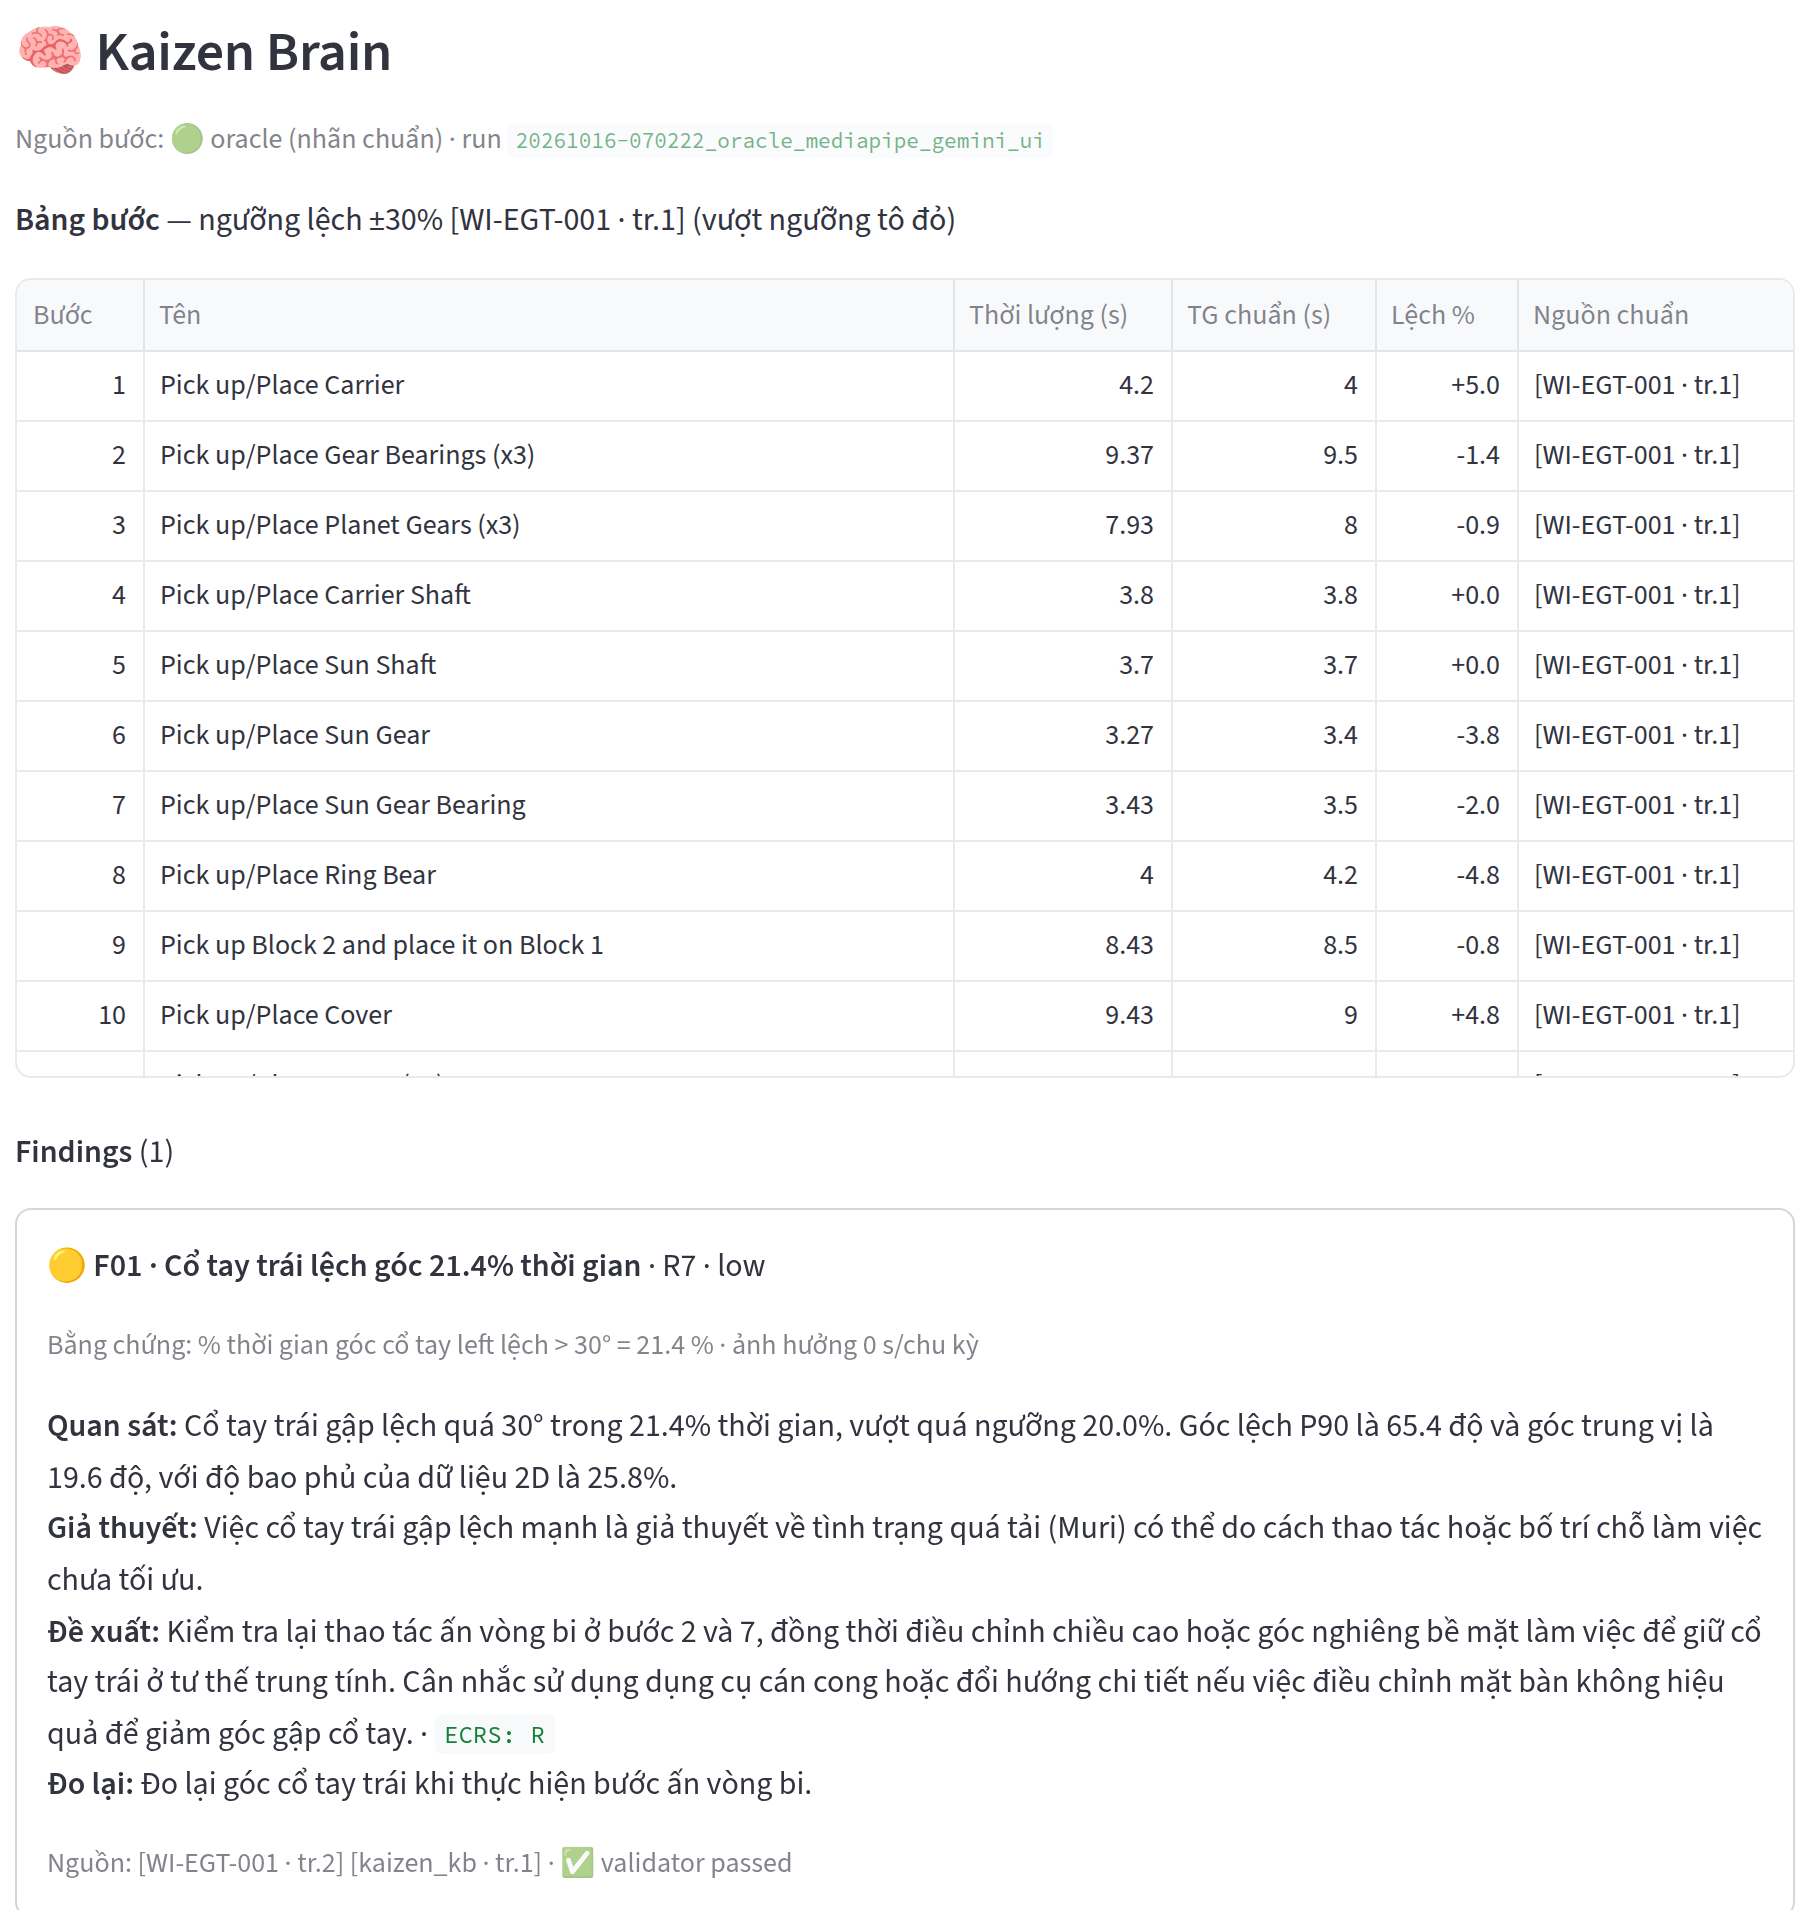
\includegraphics[width=0.75\textwidth]{ui2_brain.png}
  \caption{Trang ``Kaizen Brain'' của UI: bảng bước với thời gian chuẩn và nguồn trích dẫn, cùng một phát hiện R7
  kèm giải thích LLM đã qua validator.}
  \label{fig:ui}
\end{figure}

\subsection{Model Architectures}
\label{subsec:arch}
\textbf{Pose.} \Cref{tab:pose_models} liệt kê các backend.
MediaPipe Pose Landmarker \cite{mp_pose} chạy ở chế độ video. Hand Landmarker \cite{mp_hand}
có thể chạy trên vùng vuông quanh từng cổ tay, và tay được ghép với cổ tay gần nhất.
RTMW \cite{rtmlib} chạy qua rtmlib/ONNX.
Backend \code{rtmpose-custom} nạp một RTMPose-m \cite{rtmpose} đã fine-tune và export sang ONNX
(biến môi trường \code{KAIZEN\_POSE\_ONNX}).
Mọi backend ghi ra cùng một schema \code{.npz}: \code{kpts (T,K,3), t, names, meta}.

\begin{table}[t]
\centering
\caption{Các backend ước lượng khung xương}
\label{tab:pose_models}
\footnotesize
\setlength{\tabcolsep}{3pt}
\begin{tabularx}{\columnwidth}{@{}lcXl@{}}
\toprule
Backend & Điểm & Ghi chú & Muri \\
\midrule
MediaPipe (mặc định) & 75 & 33 thân + $2\times21$ tay; CPU & có \\
RTMW-m & 133 & toàn thân COCO-WholeBody; ONNX & có \\
RTMPose-m fine-tune & 17 & COCO-17, nhãn giả Kinect; không có điểm tay & không \\
\bottomrule
\end{tabularx}
\end{table}

\textbf{Đặc trưng cho segmenter (kp\_v1).} Mỗi frame dùng $J=15$ khớp: mũi, hai vai, hai khuỷu, hai cổ tay, hai hông,
và ba điểm của mỗi bàn tay (gốc ngón giữa, đầu ngón trỏ, đầu ngón cái).
Mỗi khớp cho 7 giá trị, nên vector đặc trưng có $D=7J=105$ chiều:
\begin{itemize}
  \item toạ độ tuyệt đối $(x/W,y/H)$, vì vị trí khay cố định theo camera;
  \item toạ độ theo thân $(p-\bar p_{\text{vai}})/\lVert p_{\text{vai,L}}-p_{\text{vai,R}}\rVert$;
  \item vận tốc $\Delta(x/W,y/H)\cdot f$;
  \item mask hợp lệ (score $\ge0{,}3$).
\end{itemize}
Khớp mà model pose không có (ví dụ COCO-17 không có bàn tay) nhận giá trị 0 và mask 0, nên $D$ luôn cố định.
Đặc trưng được chuẩn hoá z-score bằng thống kê của tập train, lưu cùng model.

\textbf{MS-TCN.} \Cref{fig:mstcn} mô tả kiến trúc, theo đúng thiết kế gốc \cite{farha2019mstcn}:
$S=4$ stage, mỗi stage $L=10$ lớp residual tích chập giãn (kernel 3, dilation $2^\ell$), 64 kênh, dropout 0{,}5.
Trường tiếp nhận của mỗi stage khoảng $2^{L+1}-1=2047$ frame (ở 15\,fps tương đương khoảng 136\,s), dài hơn một chu kỳ lắp.
Stage 2..$S$ nhận softmax của stage trước. Hàm mất mát của mỗi stage là
\begin{equation}
  \mathcal{L}_s=\frac{1}{T}\sum_t -\log \hat y_{t,c_t}
  + \frac{\lambda}{TC}\sum_{t,c}\min\!\big(\Delta_{t,c}^2,\tau^2\big),
  \label{eq:mstcn_loss}
\end{equation}
với $\Delta_{t,c}=\log\hat y_{t,c}-\log\hat y_{t-1,c}$, $\lambda=0{,}15$ và $\tau=4$.
Frame không có nhãn được bỏ qua khi tính loss.
Model có khoảng \todo{số tham số, in bằng \code{sum(p.numel())}} tham số.

\begin{figure}[t]
  \centering
  \resizebox{0.8\textwidth}{!}{% Kiến trúc MS-TCN dùng cho phân đoạn bước (TikZ) — dùng trong sections/04_implementation.tex
\begin{tikzpicture}[
  font=\scriptsize,
  >={Stealth[length=1.6mm]},
  blk/.style={draw, rounded corners=1.5pt, align=center, minimum height=0.6cm, inner sep=2pt},
  conv/.style={blk, fill=blue!8, minimum width=1.0cm},
  dil/.style={blk, fill=violet!10, minimum width=0.55cm},
  st/.style={draw=gray!70, dashed, rounded corners=3pt, inner sep=4pt},
]
% đầu vào
\node[blk, fill=gray!10, align=center] (x) at (0,0) {$X\!\in\!\mathbb{R}^{105\times T}$\\kp\_v1};
% stage 1
\node[conv, right=0.35cm of x] (in1) {1$\times$1\\conv};
\node[dil, right=0.25cm of in1] (d1) {$d{=}1$};
\node[dil, right=0.1cm of d1] (d2) {$d{=}2$};
\node[right=0.05cm of d2] (dots) {$\cdots$};
\node[dil, right=0.05cm of dots] (dL) {$2^{L-1}$};
\node[conv, right=0.25cm of dL] (out1) {1$\times$1\\conv};
\node[st, fit=(in1)(out1), label={[font=\scriptsize]above:Stage 1 (dự đoán ban đầu)}] (S1) {};
\draw[->] (x) -- (in1); \draw[->] (in1) -- (d1); \draw[->] (d1) -- (d2); \draw[->] (dL) -- (out1);

% stage 2..S
\node[blk, fill=orange!10, below=0.75cm of out1, minimum width=1.4cm] (sm) {softmax};
\node[blk, fill=violet!5, left=0.35cm of sm, minimum width=3.4cm] (S2) {Stage 2 \dots{} Stage $S$ (tinh chỉnh)\\cùng cấu trúc, vào $= C$ kênh};
\node[blk, fill=green!8, left=0.35cm of S2] (y) {$\hat{Y}_S\!\in\!\mathbb{R}^{C\times T}$};
\draw[->] (out1) -- node[right]{\tiny $\hat{Y}_1$} (sm);
\draw[->] (sm) -- (S2); \draw[->] (S2) -- (y);

% chi tiết lớp giãn
\node[draw, rounded corners=2pt, fill=violet!3, align=flush left, below=0.35cm of y.south west, anchor=north west,
      text width=6.3cm] (res) {
  \textbf{Lớp residual giãn} ($d=2^{\ell}$, $\ell=0..L-1$):\\
  \quad$h \leftarrow h + \mathrm{Dropout}\big(\mathrm{Conv}_{1\times1}(\mathrm{ReLU}(\mathrm{Conv}^{d}_{3}(h)))\big)$\\
  \textbf{Loss mỗi stage:} $\mathcal{L}_s = \mathcal{L}_{CE} + \lambda\,\mathcal{L}_{T\text{-}MSE}$ (cắt ở $\tau=4$);
  tổng $\sum_{s=1}^{S}\mathcal{L}_s$.};
\end{tikzpicture}
}
  \caption{MS-TCN cho phân đoạn bước. Đầu vào là chuỗi đặc trưng kp\_v1;
  $C$ lớp tương ứng các cặp (action, repetition) cộng lớp nền.}
  \label{fig:mstcn}
\end{figure}

\textbf{LLM và embedding.} Lớp provider thống nhất hỗ trợ Gemini (mặc định \code{gemini-2.5-flash}) \cite{gemini},
Anthropic Claude (\code{claude-sonnet-4-6}), OpenAI (\code{gpt-4.1-mini}, chế độ JSON)
và provider \code{dry-run}
để chạy không cần key.
Embedding dùng model \path{intfloat/multilingual-e5-small} \cite{e5}, chạy cục bộ.
Một embedder băm $n$-gram tất định được dùng cho CI và môi trường offline.

\subsection{Datasets}
\label{subsec:data}
\textbf{HA4M} \cite{ha4m} gồm 41 người lắp (U001--U041) bộ bánh răng hành tinh theo 12 hành động
(\cref{tab:actions}), được quay bằng Azure Kinect.
Bước 00 của pipeline đọc trực tiếp dữ liệu thật để chốt schema, thay vì giả định. Kết quả:
{\raggedright
\begin{itemize}
  \item mỗi lần lắp nằm trong thư mục \code{IDU<subject>V<trial>/};
  \item ảnh Color là chuỗi PNG $2048\times1536$, tên dạng \code{FrameID<6 số>\_DeviceTimeStamp<µs>us.png};
        fps\,=\,30, xác nhận bằng trung vị $\Delta t$\,=\,33{,}33\,ms;
  \item \code{Labels.txt} có ba cột nguyên phân tách bằng dấu cách: \code{frame action\_id repetition},
        với 0 là ``don't care'';
  \item skeleton Kinect lưu dạng TSV 32 khớp, có toạ độ chiếu lên ảnh Color.
\end{itemize}
\par}
Mỗi thư mục lần lắp chiếm khoảng 18\,GB vì có đủ mọi modality, nhưng pipeline chỉ cần Color và nhãn
(thêm Skeletons cho phần fine-tune pose).
Sau khi trích keypoint, phần huấn luyện chỉ cần file \code{.npz} (khoảng 1{,}3\,MB mỗi video) và \code{Labels.txt}.

\begin{table}[t]
\centering
\caption{12 hành động HA4M và số frame của U001\_V001}
\label{tab:actions}
\footnotesize
\setlength{\tabcolsep}{3pt}
\begin{tabularx}{\columnwidth}{@{}clcr@{}}
\toprule
ID & Hành động & Lặp & Frame \\
\midrule
1 & Pick up/Place Carrier & 1 & 126 \\
2 & Pick up/Place Gear Bearings & 3 & 281 \\
3 & Pick up/Place Planet Gears & 3 & 238 \\
4 & Pick up/Place Carrier Shaft & 1 & 114 \\
5 & Pick up/Place Sun Shaft & 1 & 111 \\
6 & Pick up/Place Sun Gear & 1 & 98 \\
7 & Pick up/Place Sun Gear Bearing & 1 & 103 \\
8 & Pick up/Place Ring Bear & 1 & 120 \\
9 & Pick up Block 2, place on Block 1 & 1 & 253 \\
10 & Pick up/Place Cover & 1 & 283 \\
11 & Pick up/Place Screw & 2 & 291 \\
12 & Allen key: turn screws, return key \& EGT & 1 & 319 \\
\midrule
0 & Don't care (đầu/cuối) & -- & 90 \\
\bottomrule
\end{tabularx}
\end{table}

\textbf{Dữ liệu đã dùng.} Hiện tại có hai lần lắp của U001: V001 (2427 frame, 80{,}9\,s) và V002 (2655 frame).
Dữ liệu cho phần huấn luyện: \todo{danh sách subject/trial đã tải, ví dụ U001--U005, tổng số video, tổng số frame}.

\textbf{Cấu hình trạm.} File \code{station.yaml} khai báo 11 zone (10 khay và vùng lắp).
Mỗi zone là vùng \textit{cổ tay} khi với vào khay, không phải viền khay, và được vẽ bằng công cụ click chuột trên một frame
(\cref{fig:station}).
File còn khai báo 12 bước SOP ứng với khay đặc trưng (bước 9 không có khay), cờ VA, ROI chạy pose
và các ngưỡng ở \cref{sec:method}.

\textbf{Tri thức.} Kho tri thức gồm ba nguồn:
\code{kaizen\_kb.md} có 16 đoạn \code{[KB-xx]} (3M, 7 lãng phí, nguyên tắc Barnes, ECRS, Standardized Work, Yamazumi);
\code{sop.md} có 16 đoạn \code{[SOP-xx]} mô phỏng SOP 12 bước;
và work instruction mô phỏng \code{WI-EGT-001} (PDF 2 trang) có bảng thời gian chuẩn từng bước, ngưỡng lệch 30\%
và ngưỡng góc cổ tay 30°.

\begin{figure}[t]
  \centering
  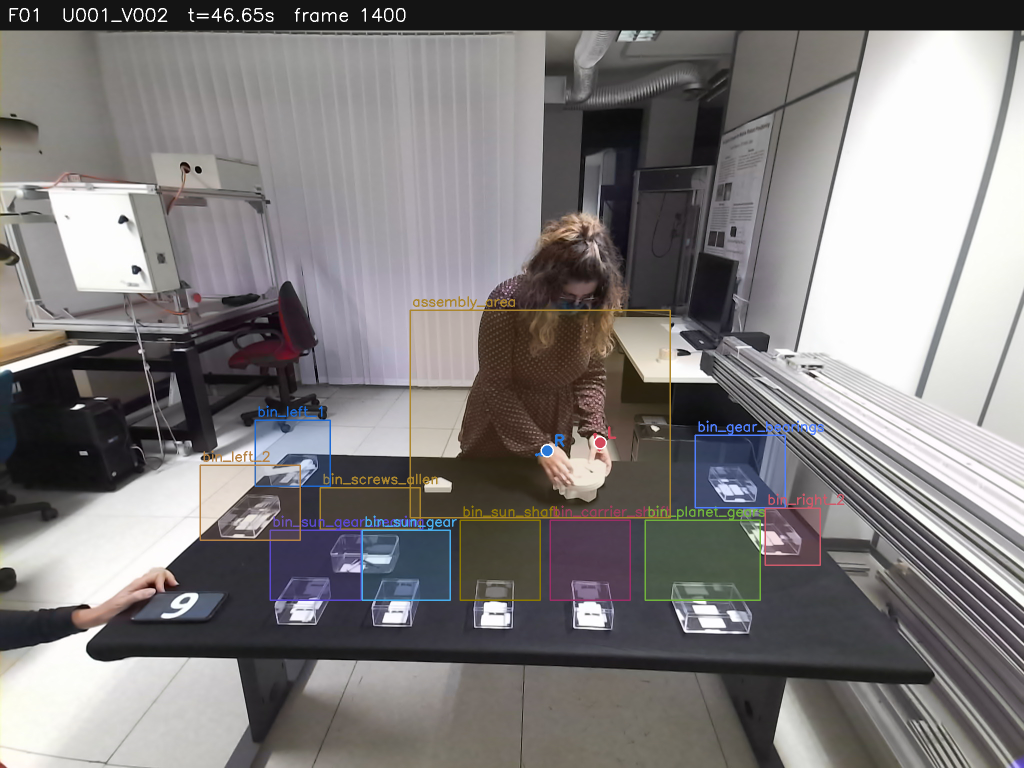
\includegraphics[width=0.85\textwidth]{evidence_F01.png}
  \caption{Trạm HA4M (U001\_V002, frame 1400) với 11 zone đã cấu hình và hai cổ tay (L/R) ước lượng bằng MediaPipe.
  Ảnh này là ảnh bằng chứng do khối 08 tự sinh cho một phát hiện.}
  \label{fig:station}
\end{figure}

\subsection{Training}
\label{subsec:training}
% ---------------------------------------------------------------
% DRAFT — điền số liệu sau khi tự chạy các lệnh trong docs/training.md
% ---------------------------------------------------------------
Huấn luyện là \textit{tuỳ chọn} và chỉ chạy khi người dùng gõ lệnh.
Khi chưa có model, pipeline vẫn dùng đường mặc định (pose pretrained, tách bước bằng quy tắc).

\textbf{Segmenter MS-TCN.} Tập dữ liệu được quét từ các cặp \code{.npz} và \code{Labels.txt}.
Nhãn được căn theo chỉ số frame của \code{.npz}.
Dữ liệu được chia train/val/test \textit{theo người lắp}, nên không người nào xuất hiện ở hai tập.
Đánh giá chéo dùng group $k$-fold theo người, hoặc leave-one-subject-out (LOSO, $k=0$).
Siêu tham số mặc định theo MS-TCN gốc (\cref{tab:hparams}).
Model được huấn luyện ở 15\,fps (lấy 1 trong 2 frame); khi dự đoán, nhãn được lặp lại về 30\,fps.
Huấn luyện dừng sớm theo F1@50 trên tập val.
Thư mục model lưu \code{model.pt}, \code{config.json} và \code{train\_log.csv}.
\code{config.json} gồm danh sách lớp, thống kê chuẩn hoá, danh sách người của từng tập, siêu tham số, epoch tốt nhất
và đánh giá mức bước trên val, theo cùng định nghĩa với khối 04.
\begin{Verbatim}[fontsize=\scriptsize,frame=single]
python -m kaizen.train.segmenter status
python -m kaizen.train.segmenter cv --folds 0
python -m kaizen.train.segmenter train --name mstcn_v1 \
       --val-subjects <S_val> --test-subjects <S_test>
\end{Verbatim}

\begin{table}[t]
\centering
\caption{Siêu tham số huấn luyện MS-TCN}
\label{tab:hparams}
\footnotesize
\begin{tabular}{@{}ll@{}}
\toprule
Tham số & Giá trị \\
\midrule
Stage / lớp / kênh & 4 / 10 / 64 \\
Dropout & 0{,}5 \\
$\lambda$ (làm mượt), $\tau$ & 0{,}15, 4 \\
Optimizer & Adam, lr $5\!\times\!10^{-4}$, weight decay $10^{-4}$ \\
Batch / epoch tối đa & 4 video / 100 \\
Early stopping & patience 20 epoch theo F1@50 (val) \\
Lấy mẫu & 1/2 (15\,fps) \\
Hậu xử lý & nhập mảnh bước $<0{,}5$\,s \\
Phần cứng & \todo{CPU/GPU, số lõi, RAM} \\
Thời gian train & \todo{phút/lần train; tổng cho CV} \\
\bottomrule
\end{tabular}
\end{table}

\todo{Đường cong loss và F1@50 (val) theo epoch, vẽ từ \code{train\_log.csv}, lưu \code{figures/train\_curve.png}
rồi bỏ comment khối figure bên dưới.}
% \begin{figure}[t]
%   \centering
%   \includegraphics[width=\columnwidth]{train_curve.png}
%   \caption{Loss train và F1@50 trên val theo epoch (MS-TCN).}
%   \label{fig:train_curve}
% \end{figure}

\textbf{Fine-tune RTMPose (nhãn giả Kinect).} Skeleton Azure Kinect đã chiếu lên ảnh Color được ánh xạ sang 17 khớp COCO.
Khớp có độ tin cậy $\ge0{,}5$ nhận visibility 2; khớp có độ tin cậy dương nhưng thấp hơn nhận visibility 1.
Cứ 15 frame lấy 1 frame; frame có ít nhất 6 khớp nhìn thấy được giữ lại.
Ảnh được crop quanh người (lề 25\%) và lưu thành JPEG kèm annotation COCO.
Model khởi tạo từ RTMPose-m pretrained trên COCO và AIC, được fine-tune 60 epoch với lr $10^{-4}$ và EMA trong MMPose
\cite{rtmpose}, rồi export ONNX bằng MMDeploy.
Nhãn giả mang theo sai số của Kinect, nhất là ở cổ tay khi bị che.
Vì vậy model fine-tune chỉ được giữ lại nếu PCK so với Kinect trên người lắp chưa thấy tốt hơn baseline.
Số liệu: \todo{số ảnh train/val, số người, thời gian train, GPU}.
